% Options for packages loaded elsewhere
\PassOptionsToPackage{unicode}{hyperref}
\PassOptionsToPackage{hyphens}{url}
%
\documentclass[
]{article}
\usepackage{amsmath,amssymb}
\usepackage{iftex}
\ifPDFTeX
  \usepackage[T1]{fontenc}
  \usepackage[utf8]{inputenc}
  \usepackage{textcomp} % provide euro and other symbols
\else % if luatex or xetex
  \usepackage{unicode-math} % this also loads fontspec
  \defaultfontfeatures{Scale=MatchLowercase}
  \defaultfontfeatures[\rmfamily]{Ligatures=TeX,Scale=1}
\fi
\usepackage{lmodern}
\ifPDFTeX\else
  % xetex/luatex font selection
\fi
% Use upquote if available, for straight quotes in verbatim environments
\IfFileExists{upquote.sty}{\usepackage{upquote}}{}
\IfFileExists{microtype.sty}{% use microtype if available
  \usepackage[]{microtype}
  \UseMicrotypeSet[protrusion]{basicmath} % disable protrusion for tt fonts
}{}
\makeatletter
\@ifundefined{KOMAClassName}{% if non-KOMA class
  \IfFileExists{parskip.sty}{%
    \usepackage{parskip}
  }{% else
    \setlength{\parindent}{0pt}
    \setlength{\parskip}{6pt plus 2pt minus 1pt}}
}{% if KOMA class
  \KOMAoptions{parskip=half}}
\makeatother
\usepackage{xcolor}
\usepackage[margin=1in]{geometry}
\usepackage{color}
\usepackage{fancyvrb}
\newcommand{\VerbBar}{|}
\newcommand{\VERB}{\Verb[commandchars=\\\{\}]}
\DefineVerbatimEnvironment{Highlighting}{Verbatim}{commandchars=\\\{\}}
% Add ',fontsize=\small' for more characters per line
\usepackage{framed}
\definecolor{shadecolor}{RGB}{248,248,248}
\newenvironment{Shaded}{\begin{snugshade}}{\end{snugshade}}
\newcommand{\AlertTok}[1]{\textcolor[rgb]{0.94,0.16,0.16}{#1}}
\newcommand{\AnnotationTok}[1]{\textcolor[rgb]{0.56,0.35,0.01}{\textbf{\textit{#1}}}}
\newcommand{\AttributeTok}[1]{\textcolor[rgb]{0.13,0.29,0.53}{#1}}
\newcommand{\BaseNTok}[1]{\textcolor[rgb]{0.00,0.00,0.81}{#1}}
\newcommand{\BuiltInTok}[1]{#1}
\newcommand{\CharTok}[1]{\textcolor[rgb]{0.31,0.60,0.02}{#1}}
\newcommand{\CommentTok}[1]{\textcolor[rgb]{0.56,0.35,0.01}{\textit{#1}}}
\newcommand{\CommentVarTok}[1]{\textcolor[rgb]{0.56,0.35,0.01}{\textbf{\textit{#1}}}}
\newcommand{\ConstantTok}[1]{\textcolor[rgb]{0.56,0.35,0.01}{#1}}
\newcommand{\ControlFlowTok}[1]{\textcolor[rgb]{0.13,0.29,0.53}{\textbf{#1}}}
\newcommand{\DataTypeTok}[1]{\textcolor[rgb]{0.13,0.29,0.53}{#1}}
\newcommand{\DecValTok}[1]{\textcolor[rgb]{0.00,0.00,0.81}{#1}}
\newcommand{\DocumentationTok}[1]{\textcolor[rgb]{0.56,0.35,0.01}{\textbf{\textit{#1}}}}
\newcommand{\ErrorTok}[1]{\textcolor[rgb]{0.64,0.00,0.00}{\textbf{#1}}}
\newcommand{\ExtensionTok}[1]{#1}
\newcommand{\FloatTok}[1]{\textcolor[rgb]{0.00,0.00,0.81}{#1}}
\newcommand{\FunctionTok}[1]{\textcolor[rgb]{0.13,0.29,0.53}{\textbf{#1}}}
\newcommand{\ImportTok}[1]{#1}
\newcommand{\InformationTok}[1]{\textcolor[rgb]{0.56,0.35,0.01}{\textbf{\textit{#1}}}}
\newcommand{\KeywordTok}[1]{\textcolor[rgb]{0.13,0.29,0.53}{\textbf{#1}}}
\newcommand{\NormalTok}[1]{#1}
\newcommand{\OperatorTok}[1]{\textcolor[rgb]{0.81,0.36,0.00}{\textbf{#1}}}
\newcommand{\OtherTok}[1]{\textcolor[rgb]{0.56,0.35,0.01}{#1}}
\newcommand{\PreprocessorTok}[1]{\textcolor[rgb]{0.56,0.35,0.01}{\textit{#1}}}
\newcommand{\RegionMarkerTok}[1]{#1}
\newcommand{\SpecialCharTok}[1]{\textcolor[rgb]{0.81,0.36,0.00}{\textbf{#1}}}
\newcommand{\SpecialStringTok}[1]{\textcolor[rgb]{0.31,0.60,0.02}{#1}}
\newcommand{\StringTok}[1]{\textcolor[rgb]{0.31,0.60,0.02}{#1}}
\newcommand{\VariableTok}[1]{\textcolor[rgb]{0.00,0.00,0.00}{#1}}
\newcommand{\VerbatimStringTok}[1]{\textcolor[rgb]{0.31,0.60,0.02}{#1}}
\newcommand{\WarningTok}[1]{\textcolor[rgb]{0.56,0.35,0.01}{\textbf{\textit{#1}}}}
\usepackage{graphicx}
\makeatletter
\def\maxwidth{\ifdim\Gin@nat@width>\linewidth\linewidth\else\Gin@nat@width\fi}
\def\maxheight{\ifdim\Gin@nat@height>\textheight\textheight\else\Gin@nat@height\fi}
\makeatother
% Scale images if necessary, so that they will not overflow the page
% margins by default, and it is still possible to overwrite the defaults
% using explicit options in \includegraphics[width, height, ...]{}
\setkeys{Gin}{width=\maxwidth,height=\maxheight,keepaspectratio}
% Set default figure placement to htbp
\makeatletter
\def\fps@figure{htbp}
\makeatother
\setlength{\emergencystretch}{3em} % prevent overfull lines
\providecommand{\tightlist}{%
  \setlength{\itemsep}{0pt}\setlength{\parskip}{0pt}}
\setcounter{secnumdepth}{-\maxdimen} % remove section numbering
\ifLuaTeX
  \usepackage{selnolig}  % disable illegal ligatures
\fi
\IfFileExists{bookmark.sty}{\usepackage{bookmark}}{\usepackage{hyperref}}
\IfFileExists{xurl.sty}{\usepackage{xurl}}{} % add URL line breaks if available
\urlstyle{same}
\hypersetup{
  pdftitle={Algal Blooms in Santa Barbara},
  hidelinks,
  pdfcreator={LaTeX via pandoc}}

\title{Algal Blooms in Santa Barbara}
\author{true}
\date{12-15-2023}

\begin{document}
\maketitle

\hypertarget{does-seasonality-have-an-effect-on-pseudo-nitzschia-algal-abundance-and-distribution}{%
\section{Does Seasonality Have an Effect on Pseudo-nitzschia Algal
Abundance and
Distribution?}\label{does-seasonality-have-an-effect-on-pseudo-nitzschia-algal-abundance-and-distribution}}

In the last few weeks, Santa Barbara has seen an unprecedented number of
marine mammals washing up on their shores. Previous research has
suggested that a particular algal species is responsible,
Pseudo-nitzschia. This particular species produces domoic acid, a
neurotoxin that causes seizures, brain damage and death in marine
mammal. These blooms can be greatly enhanced by run off, eutrophication,
and El Nino cycling where strong upwelling years foster bloom all of
which are occurring right now in Santa Barbara. These reports have also
been documented in coastal waters along the West Coast, Gulf of Mexico,
and in the Gulf of Maine affecting all animals of the food web.

The motivation for this study was formed from the questions surrounding
these blooms. What is causing them? Can we predict when they will occur
next? Can we prevent them? What conditions allow this species to thrive?

For more information regarding the data, workflow, and reproducibility
of this project please see the attached Git hub link:
\url{https://github.com/kateebeckerr/algalblooms_sb}

\hypertarget{data-descriptors}{%
\subsection{Data Descriptors:}\label{data-descriptors}}

\begin{enumerate}
\def\labelenumi{\arabic{enumi}.}
\tightlist
\item
  \textbf{Algal Events, Occurrences, and Measure}
\end{enumerate}

(2022). California Harmful Algal Bloom Monitoring and Alert Program
Data. EDI
Repository.\url{https://portal.edirepository.org/nis/metadataviewer?packageid=edi.988.8})

Relevant Variables: - Location id (Selected for Stearns Wharf) -
Organism scientific name - Organism Quantity (cells/L)

\begin{enumerate}
\def\labelenumi{\arabic{enumi}.}
\setcounter{enumi}{1}
\tightlist
\item
  \textbf{Sea Surface Temperature in Santa Barbara}
\end{enumerate}

Santa Barbara Coastal LTER, Kui, Li. (2023). Daily sea surface
temperature in Santa Barbara channel between 1982 and 2021. EDI
Repository.
URL\url{https://portal.edirepository.org/nis/mapbrowse?scope=knb-lter-sbc\&identifier=161})

Relevant Variables: - Date (2007 -\textgreater{} 2020) - Site (SITE 1
Santa Barbara) - Temperature (\href{https://www.degreesymbol.net/}{°}C)
- Latitude - Longitude

\hypertarget{relvant-libraries-and-functions}{%
\subsection{Relvant Libraries and
Functions}\label{relvant-libraries-and-functions}}

\begin{Shaded}
\begin{Highlighting}[]
\FunctionTok{library}\NormalTok{(ggplot2)}
\FunctionTok{library}\NormalTok{(tidyverse)}
\end{Highlighting}
\end{Shaded}

\begin{verbatim}
## -- Attaching core tidyverse packages ------------------------ tidyverse 2.0.0 --
## v dplyr     1.1.3     v readr     2.1.4
## v forcats   1.0.0     v stringr   1.5.0
## v lubridate 1.9.2     v tibble    3.2.1
## v purrr     1.0.2     v tidyr     1.3.0
## -- Conflicts ------------------------------------------ tidyverse_conflicts() --
## x dplyr::filter() masks stats::filter()
## x dplyr::lag()    masks stats::lag()
## i Use the conflicted package (<http://conflicted.r-lib.org/>) to force all conflicts to become errors
\end{verbatim}

\begin{Shaded}
\begin{Highlighting}[]
\FunctionTok{library}\NormalTok{(here)}
\end{Highlighting}
\end{Shaded}

\begin{verbatim}
## here() starts at /Users/katebecker/Documents/Bren/kateebeckerr.github.io
\end{verbatim}

\begin{Shaded}
\begin{Highlighting}[]
\FunctionTok{library}\NormalTok{(janitor)}
\end{Highlighting}
\end{Shaded}

\begin{verbatim}
## 
## Attaching package: 'janitor'
## 
## The following objects are masked from 'package:stats':
## 
##     chisq.test, fisher.test
\end{verbatim}

\begin{Shaded}
\begin{Highlighting}[]
\FunctionTok{library}\NormalTok{(dplyr)}
\FunctionTok{library}\NormalTok{(lubridate)}
\FunctionTok{library}\NormalTok{(sf)}
\end{Highlighting}
\end{Shaded}

\begin{verbatim}
## Linking to GEOS 3.11.0, GDAL 3.5.3, PROJ 9.1.0; sf_use_s2() is TRUE
\end{verbatim}

\begin{Shaded}
\begin{Highlighting}[]
\FunctionTok{library}\NormalTok{(terra)}
\end{Highlighting}
\end{Shaded}

\begin{verbatim}
## terra 1.7.46
## 
## Attaching package: 'terra'
## 
## The following object is masked from 'package:janitor':
## 
##     crosstab
## 
## The following object is masked from 'package:tidyr':
## 
##     extract
\end{verbatim}

\begin{Shaded}
\begin{Highlighting}[]
\FunctionTok{library}\NormalTok{(spData)}
\FunctionTok{library}\NormalTok{(spDataLarge)}
\FunctionTok{library}\NormalTok{(maps)}
\end{Highlighting}
\end{Shaded}

\begin{verbatim}
## 
## Attaching package: 'maps'
## 
## The following object is masked from 'package:purrr':
## 
##     map
\end{verbatim}

\begin{Shaded}
\begin{Highlighting}[]
\FunctionTok{library}\NormalTok{(stringr)}
\FunctionTok{library}\NormalTok{(viridis)}
\end{Highlighting}
\end{Shaded}

\begin{verbatim}
## Loading required package: viridisLite
## 
## Attaching package: 'viridis'
## 
## The following object is masked from 'package:maps':
## 
##     unemp
\end{verbatim}

\begin{Shaded}
\begin{Highlighting}[]
\FunctionTok{library}\NormalTok{(gstat)}
\FunctionTok{library}\NormalTok{(sp)}
\FunctionTok{library}\NormalTok{(automap)}
\FunctionTok{library}\NormalTok{(tufte)}
\FunctionTok{library}\NormalTok{(feasts)}
\end{Highlighting}
\end{Shaded}

\begin{verbatim}
## Loading required package: fabletools
## 
## Attaching package: 'fabletools'
## 
## The following object is masked from 'package:terra':
## 
##     interpolate
\end{verbatim}

\begin{Shaded}
\begin{Highlighting}[]
\FunctionTok{library}\NormalTok{(forecast)}
\end{Highlighting}
\end{Shaded}

\begin{verbatim}
## Registered S3 method overwritten by 'quantmod':
##   method            from
##   as.zoo.data.frame zoo
\end{verbatim}

\begin{Shaded}
\begin{Highlighting}[]
\FunctionTok{library}\NormalTok{(tsibble)}
\end{Highlighting}
\end{Shaded}

\begin{verbatim}
## 
## Attaching package: 'tsibble'
## 
## The following objects are masked from 'package:terra':
## 
##     intersect, union
## 
## The following object is masked from 'package:lubridate':
## 
##     interval
## 
## The following objects are masked from 'package:base':
## 
##     intersect, setdiff, union
\end{verbatim}

\begin{Shaded}
\begin{Highlighting}[]
\FunctionTok{library}\NormalTok{(tsibble)}
\FunctionTok{library}\NormalTok{(feasts)}
\FunctionTok{library}\NormalTok{(tmap)}
\end{Highlighting}
\end{Shaded}

\begin{verbatim}
## Breaking News: tmap 3.x is retiring. Please test v4, e.g. with
## remotes::install_github('r-tmap/tmap')
\end{verbatim}

\begin{Shaded}
\begin{Highlighting}[]
\FunctionTok{library}\NormalTok{(zoo)}
\end{Highlighting}
\end{Shaded}

\begin{verbatim}
## 
## Attaching package: 'zoo'
## 
## The following object is masked from 'package:tsibble':
## 
##     index
## 
## The following object is masked from 'package:terra':
## 
##     time<-
## 
## The following objects are masked from 'package:base':
## 
##     as.Date, as.Date.numeric
\end{verbatim}

\begin{Shaded}
\begin{Highlighting}[]
\FunctionTok{library}\NormalTok{(spData)}
\FunctionTok{library}\NormalTok{(purrr)}
\FunctionTok{library}\NormalTok{(forcats)}
\FunctionTok{library}\NormalTok{(readr)}
\FunctionTok{library}\NormalTok{(gt)}
\end{Highlighting}
\end{Shaded}

\hypertarget{setting-the-working-directory}{%
\subsection{Setting The Working
Directory}\label{setting-the-working-directory}}

\begin{Shaded}
\begin{Highlighting}[]
\FunctionTok{rm}\NormalTok{(}\AttributeTok{list =} \FunctionTok{ls}\NormalTok{())}
\NormalTok{here}\SpecialCharTok{::}\FunctionTok{i\_am}\NormalTok{(}\StringTok{"algae\_temp\_analysis.qmd"}\NormalTok{)}
\end{Highlighting}
\end{Shaded}

\begin{verbatim}
## here() starts at /Users/katebecker/Documents/Bren/kateebeckerr.github.io/posts/Algae_Stats
\end{verbatim}

\begin{Shaded}
\begin{Highlighting}[]
\FunctionTok{setwd}\NormalTok{(}\FunctionTok{here}\NormalTok{())}
\end{Highlighting}
\end{Shaded}

\hypertarget{data-read-in}{%
\subsection{Data Read In}\label{data-read-in}}

\begin{Shaded}
\begin{Highlighting}[]
\NormalTok{algal\_events }\OtherTok{\textless{}{-}} \FunctionTok{read\_csv}\NormalTok{(}\StringTok{"/Users/katebecker/Documents/Bren/Fall\_Q/EDS\_222/ final\_proj/algalblooms\_sb/data/edi/event.csv"}\NormalTok{)}
\end{Highlighting}
\end{Shaded}

\begin{verbatim}
## Rows: 4448 Columns: 12
## -- Column specification --------------------------------------------------------
## Delimiter: ","
## chr  (6): id, eventID, geodeticDatum, countryCode, locationID, eventRemarks
## dbl  (5): decimalLatitude, decimalLongitude, minimumDepthInMeters, maximumDe...
## dttm (1): eventDate
## 
## i Use `spec()` to retrieve the full column specification for this data.
## i Specify the column types or set `show_col_types = FALSE` to quiet this message.
\end{verbatim}

\begin{Shaded}
\begin{Highlighting}[]
\NormalTok{algal\_measure }\OtherTok{\textless{}{-}} \FunctionTok{read\_csv}\NormalTok{(}\StringTok{"/Users/katebecker/Documents/Bren/Fall\_Q/EDS\_222/ final\_proj/algalblooms\_sb/data/edi/extendedmeasurementorfact.csv"}\NormalTok{)}
\end{Highlighting}
\end{Shaded}

\begin{verbatim}
## Rows: 44955 Columns: 7
## -- Column specification --------------------------------------------------------
## Delimiter: ","
## chr (6): id, measurementType, measurementID, measurementTypeID, measurementU...
## dbl (1): measurementValue
## 
## i Use `spec()` to retrieve the full column specification for this data.
## i Specify the column types or set `show_col_types = FALSE` to quiet this message.
\end{verbatim}

\begin{Shaded}
\begin{Highlighting}[]
\NormalTok{algal\_occurence }\OtherTok{\textless{}{-}} \FunctionTok{read\_csv}\NormalTok{(}\StringTok{"/Users/katebecker/Documents/Bren/Fall\_Q/EDS\_222/ final\_proj/algalblooms\_sb/data/edi/occurrence.csv"}\NormalTok{)}
\end{Highlighting}
\end{Shaded}

\begin{verbatim}
## Rows: 28892 Columns: 11
## -- Column specification --------------------------------------------------------
## Delimiter: ","
## chr (10): id, basisOfRecord, organismName, organismQuantityType, occurrenceI...
## dbl  (1): organismQuantity
## 
## i Use `spec()` to retrieve the full column specification for this data.
## i Specify the column types or set `show_col_types = FALSE` to quiet this message.
\end{verbatim}

\begin{Shaded}
\begin{Highlighting}[]
\NormalTok{sst }\OtherTok{\textless{}{-}} \FunctionTok{read\_csv}\NormalTok{(}\StringTok{"/Users/katebecker/Documents/Bren/Fall\_Q/EDS\_222/ final\_proj/algalblooms\_sb/data/sst/sst\_original\_data.csv"}\NormalTok{)}
\end{Highlighting}
\end{Shaded}

\begin{verbatim}
## Rows: 262944 Columns: 5
## -- Column specification --------------------------------------------------------
## Delimiter: ","
## chr  (1): site
## dbl  (3): latitude, longitude, temp
## date (1): date
## 
## i Use `spec()` to retrieve the full column specification for this data.
## i Specify the column types or set `show_col_types = FALSE` to quiet this message.
\end{verbatim}

\hypertarget{analysis}{%
\section{Analysis}\label{analysis}}

\hypertarget{data-exploration}{%
\subsection{Data Exploration}\label{data-exploration}}

\begin{Shaded}
\begin{Highlighting}[]
\CommentTok{\#Algal Events }
\CommentTok{\#head(algal\_events)}
\CommentTok{\#shape(algal\_events)}
\CommentTok{\#class(algal\_events)}

\CommentTok{\#Algal Meausre}
\CommentTok{\#head(algal\_measure)}
\CommentTok{\#shape(algal\_measure)}
\CommentTok{\#class(algal\_measure)}


\CommentTok{\# Algal Occurence}
\CommentTok{\#shape(algal\_occurence)}
\CommentTok{\#head(algal\_occurence)}
\CommentTok{\#class(algal\_measure)}
\CommentTok{\#shape(algal\_occurence)}

\CommentTok{\#SST}
\CommentTok{\#head(sst)}
\CommentTok{\#class(sst)}
\CommentTok{\#shape(sst)}
\CommentTok{\#class(sst)}
\end{Highlighting}
\end{Shaded}

\hypertarget{data-wrangling}{%
\subsection{Data Wrangling}\label{data-wrangling}}

\hypertarget{algae-data}{%
\subsubsection{Algae Data}\label{algae-data}}

Grouping by organism and filtering for the toxic algae Pseudo nitzschia
and specific location will also be filtered for ``Stearns Wharf''.

\begin{Shaded}
\begin{Highlighting}[]
\NormalTok{names\_algae }\OtherTok{\textless{}{-}}\NormalTok{ algal\_occurence }\SpecialCharTok{\%\textgreater{}\%}
  \FunctionTok{group\_by}\NormalTok{(organismName) }\SpecialCharTok{\%\textgreater{}\%} \CommentTok{\#grouping by organism name}
  \FunctionTok{na.omit}\NormalTok{() }\CommentTok{\#omitting na}

\NormalTok{pseudo\_algae }\OtherTok{\textless{}{-}}\NormalTok{ algal\_occurence }\SpecialCharTok{\%\textgreater{}\%}
  \FunctionTok{filter}\NormalTok{(organismName }\SpecialCharTok{==} \StringTok{"Pseudo\_nitzschia\_seriata\_group"}\NormalTok{) }\CommentTok{\#filter for toxic algal species}

\NormalTok{join }\OtherTok{\textless{}{-}} \FunctionTok{left\_join}\NormalTok{(pseudo\_algae, algal\_events, }\AttributeTok{by =} \StringTok{"id"}\NormalTok{) }\CommentTok{\#left join algal\_events into pseuo\_algae by ID}

\NormalTok{join\_stearns }\OtherTok{\textless{}{-}}\NormalTok{ join }\SpecialCharTok{\%\textgreater{}\%}
  \FunctionTok{filter}\NormalTok{(locationID }\SpecialCharTok{==} \StringTok{"HABs{-}StearnsWharf"}\NormalTok{) }\SpecialCharTok{\%\textgreater{}\%} \CommentTok{\#filter for location ID of Stearns Wharf in SB}
  \FunctionTok{mutate}\NormalTok{(}\AttributeTok{year =} \FunctionTok{format}\NormalTok{(eventDate, }\StringTok{"\%Y"}\NormalTok{)) }\CommentTok{\#Create a year column by extracting it from eventDate variable}
\end{Highlighting}
\end{Shaded}

\hypertarget{sst-data}{%
\subsubsection{SST Data}\label{sst-data}}

Filtering for data between the years 2007 and 2022 as well as for
``SITE1'' Stearns Wharf

\begin{Shaded}
\begin{Highlighting}[]
\NormalTok{sst\_filter }\OtherTok{\textless{}{-}}\NormalTok{ sst }\SpecialCharTok{\%\textgreater{}\%}
  \FunctionTok{mutate}\NormalTok{(}\AttributeTok{year =} \FunctionTok{format}\NormalTok{(date, }\StringTok{"\%Y"}\NormalTok{)) }\CommentTok{\#adds a new column named year to the sst dataframe by extracting the year value from date }

\NormalTok{updated\_sst }\OtherTok{\textless{}{-}}\NormalTok{ sst\_filter }\SpecialCharTok{\%\textgreater{}\%} \CommentTok{\#creates a new df filtering only rows where year column is greater than or equal to 2007 and less than or equal to 2022}
  \FunctionTok{filter}\NormalTok{(year }\SpecialCharTok{\textgreater{}=} \DecValTok{2007} \SpecialCharTok{\&}\NormalTok{ year }\SpecialCharTok{\textless{}=} \DecValTok{2022}\NormalTok{)}

\NormalTok{sst\_filter }\OtherTok{\textless{}{-}}\NormalTok{ sst\_filter }\SpecialCharTok{\%\textgreater{}\%}
  \FunctionTok{mutate}\NormalTok{(}\AttributeTok{index =} \FunctionTok{as.Date}\NormalTok{(date)) }\CommentTok{\#adds a new column, index, which is created by converting the date column to a date object}

\NormalTok{sst\_filter }\OtherTok{\textless{}{-}} \FunctionTok{na.omit}\NormalTok{(sst\_filter) }\CommentTok{\#omits na}

\NormalTok{sst\_filter }\OtherTok{\textless{}{-}}\NormalTok{ sst\_filter }\SpecialCharTok{\%\textgreater{}\%}
  \FunctionTok{arrange}\NormalTok{(index) }\CommentTok{\#sorts dataframe by index column}

\NormalTok{sst\_filter }\OtherTok{\textless{}{-}}\NormalTok{ sst\_filter }\SpecialCharTok{\%\textgreater{}\%}
  \FunctionTok{mutate}\NormalTok{(}\AttributeTok{index =} \FunctionTok{as.Date}\NormalTok{(date),}
         \AttributeTok{temp =} \FunctionTok{as.numeric}\NormalTok{(temp)) }\CommentTok{\#converting temp column to numeric}

\CommentTok{\#Repeats steps but for SITE1 exlusively }
\NormalTok{sst\_site1 }\OtherTok{\textless{}{-}}\NormalTok{ sst\_filter }\SpecialCharTok{\%\textgreater{}\%}
  \FunctionTok{filter}\NormalTok{(site }\SpecialCharTok{==} \StringTok{"SITE1"}\NormalTok{) }\CommentTok{\#filtering for SITE1 (Stearns Warf)}

\NormalTok{sst\_filter1 }\OtherTok{\textless{}{-}}\NormalTok{ sst\_site1 }\SpecialCharTok{\%\textgreater{}\%}
  \FunctionTok{mutate}\NormalTok{(}\AttributeTok{index =} \FunctionTok{as.Date}\NormalTok{(date))  }\CommentTok{\#adds a new column, index, which is creaed by converting date column to a date object}

\NormalTok{sst\_filter1 }\OtherTok{\textless{}{-}} \FunctionTok{na.omit}\NormalTok{(sst\_filter1) }\CommentTok{\#omits na}

\NormalTok{sst\_filter }\OtherTok{\textless{}{-}}\NormalTok{ sst\_filter1 }\SpecialCharTok{\%\textgreater{}\%}
  \FunctionTok{arrange}\NormalTok{(index) }\CommentTok{\#sorts df by index column}

\NormalTok{sst\_filter1 }\OtherTok{\textless{}{-}}\NormalTok{ sst\_filter1 }\SpecialCharTok{\%\textgreater{}\%}
  \FunctionTok{mutate}\NormalTok{(}\AttributeTok{index =} \FunctionTok{as.Date}\NormalTok{(date),}
         \AttributeTok{temp =} \FunctionTok{as.numeric}\NormalTok{(temp)) }\CommentTok{\#converting temp into a numeric}
\end{Highlighting}
\end{Shaded}

\hypertarget{joining-data}{%
\subsection{Joining Data}\label{joining-data}}

\begin{Shaded}
\begin{Highlighting}[]
\NormalTok{date\_join\_stearns }\OtherTok{\textless{}{-}} \FunctionTok{left\_join}\NormalTok{(join\_stearns, updated\_sst, }\AttributeTok{by =}\StringTok{"year"}\NormalTok{) }\CommentTok{\#join into join\_stearns by id}
\end{Highlighting}
\end{Shaded}

\begin{verbatim}
## Warning in left_join(join_stearns, updated_sst, by = "year"): Detected an unexpected many-to-many relationship between `x` and `y`.
## i Row 1 of `x` matches multiple rows in `y`.
## i Row 6571 of `y` matches multiple rows in `x`.
## i If a many-to-many relationship is expected, set `relationship =
##   "many-to-many"` to silence this warning.
\end{verbatim}

\begin{Shaded}
\begin{Highlighting}[]
\NormalTok{join }\OtherTok{\textless{}{-}}\NormalTok{ join[}\FunctionTok{complete.cases}\NormalTok{(join}\SpecialCharTok{$}\NormalTok{decimalLatitude, join}\SpecialCharTok{$}\NormalTok{decimalLongitude), ] }\CommentTok{\#filters rows in join dataframe whre both lat and long are not missing}
\NormalTok{join\_sf }\OtherTok{\textless{}{-}} \FunctionTok{st\_as\_sf}\NormalTok{(join, }\AttributeTok{coords =} \FunctionTok{c}\NormalTok{(}\StringTok{"decimalLatitude"}\NormalTok{, }\StringTok{"decimalLongitude"}\NormalTok{), }\AttributeTok{crs =} \DecValTok{4326}\NormalTok{) }\CommentTok{\#converts join df into a spatial feature and uses crs 4326}

\NormalTok{date\_join\_stearns }\OtherTok{\textless{}{-}}\NormalTok{ date\_join\_stearns }\SpecialCharTok{\%\textgreater{}\%}
  \FunctionTok{mutate}\NormalTok{(}\AttributeTok{y\_m =} \FunctionTok{yearmonth}\NormalTok{(date)) }\SpecialCharTok{\%\textgreater{}\%} \CommentTok{\#adds a y\_m columm representing year and month of the date column }
  \FunctionTok{filter}\NormalTok{(}\SpecialCharTok{!}\FunctionTok{is.na}\NormalTok{(date)) }\CommentTok{\#filters out rows where date is not missing }
\end{Highlighting}
\end{Shaded}

\hypertarget{data-exploration-1}{%
\subsection{Data Exploration}\label{data-exploration-1}}

\hypertarget{plotting-temp-and-date-relationship}{%
\subsubsection{Plotting Temp and Date
Relationship}\label{plotting-temp-and-date-relationship}}

\begin{Shaded}
\begin{Highlighting}[]
\NormalTok{linear\_model }\OtherTok{\textless{}{-}} \FunctionTok{lm}\NormalTok{(temp }\SpecialCharTok{\textasciitilde{}}\NormalTok{ date, }\AttributeTok{data =}\NormalTok{ updated\_sst) }\CommentTok{\#fits a linear model}
\NormalTok{slope }\OtherTok{\textless{}{-}} \FunctionTok{coef}\NormalTok{(linear\_model)[}\DecValTok{2}\NormalTok{] }\CommentTok{\#extracts slope coefficient for data variable from linear model }

\CommentTok{\#we\textquotesingle{}ve all see this general trend, showing seasonal oscillations}
\FunctionTok{ggplot}\NormalTok{(}\AttributeTok{data =}\NormalTok{ updated\_sst, }\FunctionTok{aes}\NormalTok{(}\AttributeTok{x =}\NormalTok{ date, }\AttributeTok{y =}\NormalTok{ temp)) }\SpecialCharTok{+}
  \FunctionTok{geom\_point}\NormalTok{(}\AttributeTok{color =} \StringTok{"\#726161"}\NormalTok{, }\AttributeTok{size =} \FloatTok{0.25}\NormalTok{) }\SpecialCharTok{+}
  \FunctionTok{geom\_smooth}\NormalTok{(}\AttributeTok{method =} \StringTok{"lm"}\NormalTok{, }\AttributeTok{se =} \ConstantTok{FALSE}\NormalTok{, }\AttributeTok{color =} \StringTok{"red"}\NormalTok{) }\SpecialCharTok{+} \CommentTok{\#adds a treadline to plot using linear model }
  \FunctionTok{labs}\NormalTok{(}\AttributeTok{x =} \StringTok{"Time"}\NormalTok{, }
       \AttributeTok{y =} \StringTok{"Sea Surface Temperature (°C)"}\NormalTok{) }\SpecialCharTok{+} 
  \FunctionTok{ggtitle}\NormalTok{(}\StringTok{"Sea Surface Temperature Trend Over the Last 15 Years"}\NormalTok{)}
\end{Highlighting}
\end{Shaded}

\begin{verbatim}
## `geom_smooth()` using formula = 'y ~ x'
\end{verbatim}

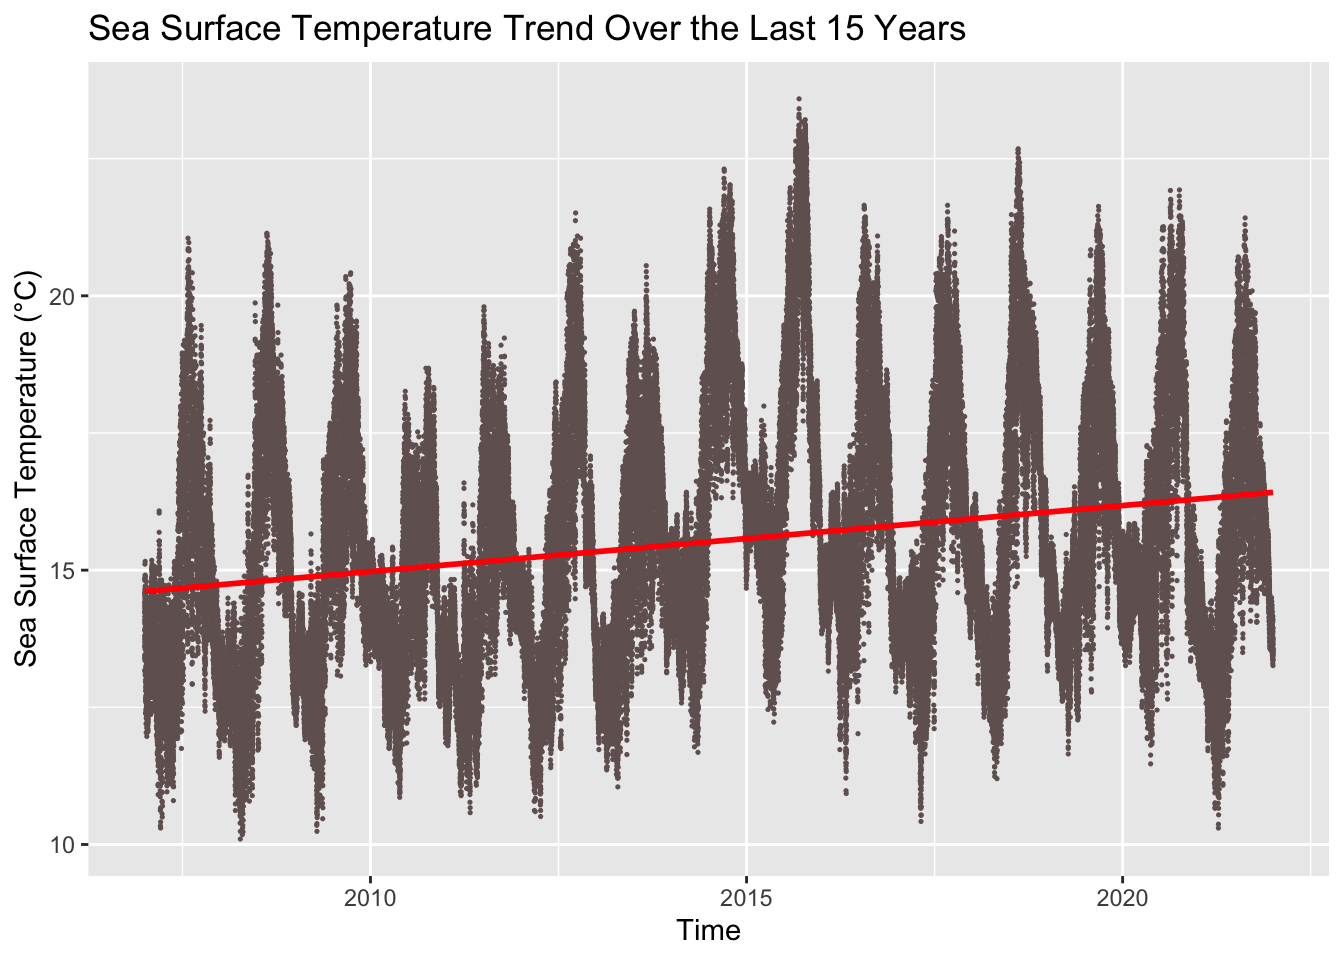
\includegraphics{algae_temp_analysis_files/figure-latex/unnamed-chunk-8-1.pdf}

Sea surface temperature over the last 15 years shows a prominent trend.
There's clear seasonality and a steady upward trend likely to continue
in the following years.

\hypertarget{statistical-analysis}{%
\subsection{Statistical Analysis}\label{statistical-analysis}}

H0: Seasonality does affect algal bloom abundance and distribution

HA: Seasonality does not affect algal bloom abundance and Distribution

\hypertarget{linear-regression}{%
\subsubsection{Linear Regression}\label{linear-regression}}

\begin{Shaded}
\begin{Highlighting}[]
\FunctionTok{summary}\NormalTok{(}\FunctionTok{lm}\NormalTok{(temp }\SpecialCharTok{\textasciitilde{}}\NormalTok{ date, }\AttributeTok{data =}\NormalTok{ sst\_filter))}
\end{Highlighting}
\end{Shaded}

\begin{verbatim}
## 
## Call:
## lm(formula = temp ~ date, data = sst_filter)
## 
## Residuals:
##     Min      1Q  Median      3Q     Max 
## -4.3314 -1.2862 -0.2467  1.1287  6.9665 
## 
## Coefficients:
##              Estimate Std. Error t value Pr(>|t|)    
## (Intercept) 1.471e+01  4.239e-02 347.041   <2e-16 ***
## date        2.176e-06  3.412e-06   0.638    0.524    
## ---
## Signif. codes:  0 '***' 0.001 '**' 0.01 '*' 0.05 '.' 0.1 ' ' 1
## 
## Residual standard error: 1.739 on 14606 degrees of freedom
## Multiple R-squared:  2.784e-05,  Adjusted R-squared:  -4.063e-05 
## F-statistic: 0.4066 on 1 and 14606 DF,  p-value: 0.5237
\end{verbatim}

A p-value of 2.2×10−162.2×10−16 is extremely small and essentially zero.
In statistical hypothesis testing, a common significance level (alpha)
is 0.05. If the p-value is less than 0.05, the null hypothesis is
typically rejected, suggesting that there is evidence to support the
alternative hypothesis. In this case, with a p-value much smaller than
0.05 (specifically, 2.2×10−162.2×10−16), it indicates strong evidence
against the null hypothesis. You would generally conclude that there is
a statistically significant relationship between the independent
variable(s) in your linear regression model and the dependent variable
but this value and the coefficients don't correlate to the rrange of
this data.

In summary, based on the p-value provided we can reject null hypothesis,
supporting the idea that there is a statistically significant
relationship in the linear regression model. Unfortunately, due to how
small the p-value is it should cause pause.

\hypertarget{decomposition}{%
\subsubsection{Decomposition}\label{decomposition}}

Isolating each component of the time series visually and quantitatively

\begin{Shaded}
\begin{Highlighting}[]
\NormalTok{decomp\_stearn }\OtherTok{\textless{}{-}}\NormalTok{ date\_join\_stearns }\SpecialCharTok{\%\textgreater{}\%}
  \FunctionTok{filter}\NormalTok{(}\SpecialCharTok{!}\FunctionTok{is.na}\NormalTok{(date)) }\SpecialCharTok{\%\textgreater{}\%}  \CommentTok{\#filters out where date is not missing}
  \FunctionTok{mutate}\NormalTok{(}\AttributeTok{y\_m =} \FunctionTok{yearmonth}\NormalTok{(date)) }\SpecialCharTok{\%\textgreater{}\%} \CommentTok{\#add a new column y\_m representing year and month from date column}
  \FunctionTok{group\_by}\NormalTok{(y\_m) }\SpecialCharTok{\%\textgreater{}\%} \CommentTok{\#groups data by year and month}
  \FunctionTok{summarise}\NormalTok{(}\AttributeTok{total\_quant =} \FunctionTok{sum}\NormalTok{(organismQuantity, }\AttributeTok{na.rm =} \ConstantTok{TRUE}\NormalTok{)) }\SpecialCharTok{\%\textgreater{}\%} \CommentTok{\#calculates total quantity of organism for each group ignoring missing values}
  \FunctionTok{mutate}\NormalTok{(}\AttributeTok{total\_quant =} \FunctionTok{na.approx}\NormalTok{(total\_quant)) }\SpecialCharTok{\%\textgreater{}\%} \CommentTok{\#interpolates missing values in total\_quant column}
  \FunctionTok{as\_tsibble}\NormalTok{(}\AttributeTok{index =}\NormalTok{ y\_m) }\CommentTok{\#converts data to a tsibble}
\end{Highlighting}
\end{Shaded}

\begin{Shaded}
\begin{Highlighting}[]
\NormalTok{decomp\_stearn }\SpecialCharTok{\%\textgreater{}\%} \FunctionTok{model}\NormalTok{( }\CommentTok{\#specifies the STL decomposition time series model }
    \FunctionTok{STL}\NormalTok{(total\_quant)}
\NormalTok{  ) }\SpecialCharTok{\%\textgreater{}\%}
  \FunctionTok{components}\NormalTok{() }\SpecialCharTok{\%\textgreater{}\%} \CommentTok{\#extracts components (trend, seasonality, and remainder) from decomposition}
  \FunctionTok{autoplot}\NormalTok{() }\SpecialCharTok{+} \CommentTok{\#creates a visualization}
  \FunctionTok{labs}\NormalTok{(}\AttributeTok{title =} \StringTok{"Stearns Warf, Santa Barbara"}\NormalTok{)}
\end{Highlighting}
\end{Shaded}

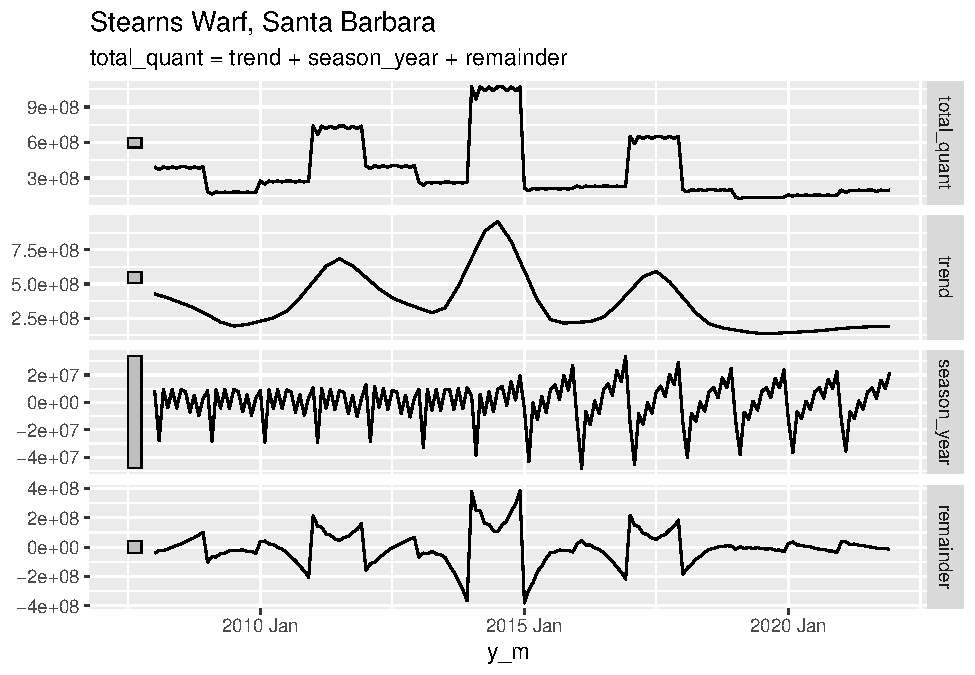
\includegraphics{algae_temp_analysis_files/figure-latex/unnamed-chunk-11-1.pdf}

*Data ends in 2022 so we can only infer what the trend looks like as it
approaches 2024

In 2015, the US west coast suffered the worst, on record, domoic event
and this is evident in the prominent spike shown in this graph at the
2015 time stamp. This suggests a correlation between organism quantity
and time of year. This graph also shows clear seasonality with a
peculiar increase in magnitude of the season\_year oscillations after
2015. It should also be noted that the residuals show a general trend
which suggests that there are other drivers to this analysis that aren't
accounted for. Finally, after examining the size of the grey bars, the
long run trend and the residuals appear to be important in driving the
overall variation in algae count.

\hypertarget{multiple-linear-regression}{%
\subsection{Multiple Linear
Regression}\label{multiple-linear-regression}}

\begin{Shaded}
\begin{Highlighting}[]
\NormalTok{date\_join\_stearns }\OtherTok{\textless{}{-}}\NormalTok{ date\_join\_stearns }\SpecialCharTok{\%\textgreater{}\%}
  \FunctionTok{mutate}\NormalTok{(}\AttributeTok{year =} \FunctionTok{format}\NormalTok{(y\_m, }\StringTok{"\%Y"}\NormalTok{)) }\CommentTok{\#extracts year from y\_m  column}

\NormalTok{mod }\OtherTok{\textless{}{-}} \FunctionTok{lm}\NormalTok{(organismQuantity }\SpecialCharTok{\textasciitilde{}}\NormalTok{ temp }\SpecialCharTok{+}\NormalTok{ year, }\AttributeTok{data =}\NormalTok{ date\_join\_stearns) }\CommentTok{\#fits a linear regression model where organism quantity is dependent and temp and year are independent variables }
\FunctionTok{summary}\NormalTok{(mod) }\CommentTok{\#summary statistics}
\end{Highlighting}
\end{Shaded}

\begin{verbatim}
## 
## Call:
## lm(formula = organismQuantity ~ temp + year, data = date_join_stearns)
## 
## Residuals:
##    Min     1Q Median     3Q    Max 
## -38427 -10693  -6358  -1796 338772 
## 
## Coefficients:
##               Estimate Std. Error t value Pr(>|t|)    
## (Intercept)  2.826e+04  1.548e+02  182.58   <2e-16 ***
## temp        -3.622e-10  8.384e+00    0.00        1    
## year2009    -2.190e+04  1.120e+02 -195.47   <2e-16 ***
## year2010    -1.756e+04  1.141e+02 -153.99   <2e-16 ***
## year2011    -2.278e+03  1.121e+02  -20.33   <2e-16 ***
## year2012    -1.435e+04  1.117e+02 -128.48   <2e-16 ***
## year2013    -1.877e+04  1.124e+02 -167.01   <2e-16 ***
## year2014     1.017e+04  1.135e+02   89.57   <2e-16 ***
## year2015    -2.097e+04  1.135e+02 -184.70   <2e-16 ***
## year2016    -2.028e+04  1.120e+02 -181.01   <2e-16 ***
## year2017    -5.305e+03  1.123e+02  -47.26   <2e-16 ***
## year2018    -2.121e+04  1.125e+02 -188.47   <2e-16 ***
## year2019    -2.357e+04  1.119e+02 -210.65   <2e-16 ***
## year2020    -2.029e+04  1.205e+02 -168.38   <2e-16 ***
## year2021    -2.118e+04  1.126e+02 -188.20   <2e-16 ***
## ---
## Signif. codes:  0 '***' 0.001 '**' 0.01 '*' 0.05 '.' 0.1 ' ' 1
## 
## Residual standard error: 37230 on 4389897 degrees of freedom
## Multiple R-squared:  0.0662, Adjusted R-squared:  0.0662 
## F-statistic: 2.223e+04 on 14 and 4389897 DF,  p-value: < 2.2e-16
\end{verbatim}

The p-value remains the same and the coefficients again don't make much
sense in terms of the data making it difficult to accept or reject the
null.

\hypertarget{autocorrelation}{%
\subsection{Autocorrelation}\label{autocorrelation}}

In order to extract insights into seasonality and periodicity in time
series data, Autocorrelation works well. Interpretation of the ACF plot
involves examining the heights and patterns of the bars or spikes. The
bars that extend beyond the shaded region indicate statistically
significant correlations. Interpretation of this provides a graphical
representation of how the values of a time series are correlated with
their own past values at different lags. By specifying
\textbf{\texttt{lag.max\ =\ 52}}, it constructs an autocorrelation up to
a lag of 52 time points.

\begin{Shaded}
\begin{Highlighting}[]
\FunctionTok{acf}\NormalTok{(decomp\_stearn}\SpecialCharTok{$}\NormalTok{total\_quant, }\AttributeTok{lag.max=}\DecValTok{52}\NormalTok{) }
\end{Highlighting}
\end{Shaded}

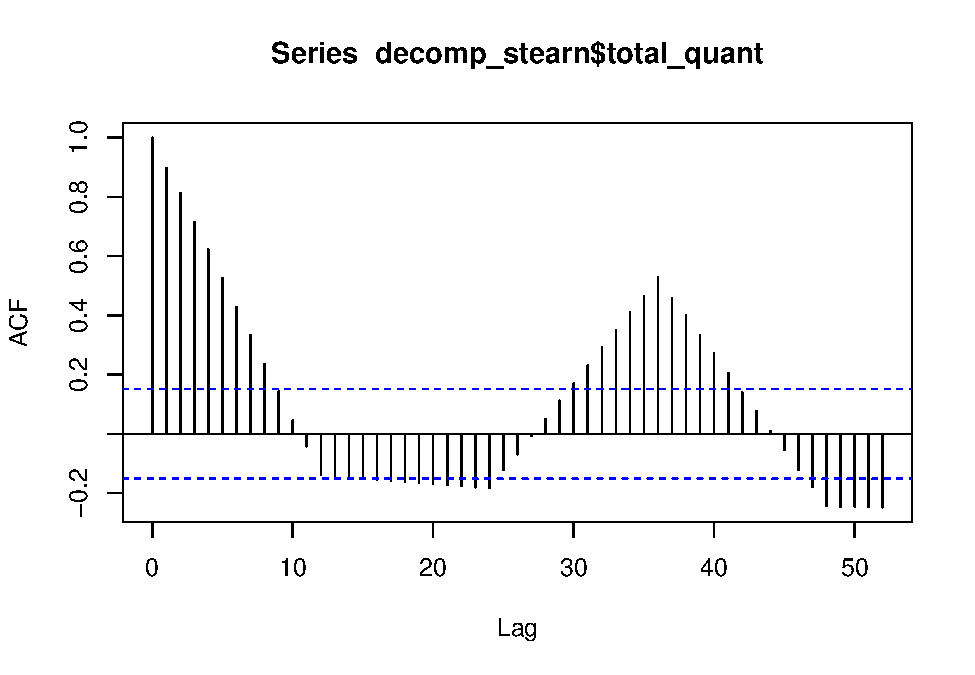
\includegraphics{algae_temp_analysis_files/figure-latex/unnamed-chunk-13-1.pdf}

To assess the nature of seasonality, a 52 week annual window of time was
used. This autocorrelation shows values close to 1 (such as lag 1)
showing strong positive correlation with past values. There is also
evident toughs and peaks representing a repeating pattern and
seasonality as well as statistically significant values concluding that
the observed correlations are unlikely due to random chance.

\hypertarget{findings}{%
\subsection{Findings}\label{findings}}

Although this study shows seasonal trends between temperature and time
over the last 15 years, the linear regression models that were run don't
provide sufficient p-values or coefficients to confidently accept the
null that seasonality does in fact affect algal bloom abundance and
distribution. Further analysis is required.

\end{document}
